\documentclass[a4paper,11pt]{article}

\title{\S10. Importing Figures}
\author{Andrew Brendon-Penn}

\usepackage{amsmath}
\usepackage{amssymb}
\usepackage{amsfonts}
\usepackage{gensymb} % used for \degree

% packages needed to make diagrams work
\usepackage{graphicx}    	% very important, heavily used for figures
\usepackage{subcaption}  	% used to allow captions to subfigures
\usepackage{wrapfig}		% used for wrapping text around figures

\begin{document}
\maketitle

\section{Figures}

I would like to import a figure.

\begin{figure}[hbtp]
	\centering % centers the picture horizontally
	\includegraphics[width=5in]{IVT.jpg} % optional argument could be height = , scale = etc. and can take in units mm, cm, in, pt, em, mu,...
	\caption{Illustration of Intermediate Value Theorem}
	\label{fig:IVT}  % put the label on the caption, as this is what has been numbered.
\end{figure}
%
Because it is bad style to add a figure without referring to it in the text, then I should add a caption (which is automatically numbered) and a label so that I can now  refer to (poor quality) figure \ref{fig:IVT} in my text. I might have to compile twice to make this work!

\pagebreak

\section{Positioning}

\LaTeX will try to do a good job for you choosing the position of your diagram. However, you need to allow it to do so.  We do this in the optional argument of the figure environment by specifying which options \LaTeX is allowed to consider. For best results, usually we write hbtp (the order of these letters does not matter). These stand for
\begin{description}
\item{\textbf{h}ere} --- approximately corresponding to this point in  source code
\item{\textbf{b}ottom}  --- at the bottom of the page
\item{\textbf{t}op} --- at the top of the page
\item{\textbf{p}age of figures} --- on a page with only figures on
\end{description}
% there are more options, read more here on the wikibook: https://en.wikibooks.org/wiki/LaTeX/Floats,_Figures_and_Captions

Failure to give all these options can lead to poor choices. For example, in \ref{fig:IVTnoposition}, I've not specified any positioning information and the figure is not where I expect it to be.
%
\begin{figure}
	\centering % centers the picture horizontally
	\includegraphics[width=4in]{IVT.jpg} % optional argument could be height = , scale = etc. and can take in units mm, cm, in, pt, em, mu,...
	\caption{Illustration of Intermediate Value Theorem}
	\label{fig:IVTnoposition}
\end{figure}
%

If you are not satisfied with the figure  placement, then often it's worth going back to your image and trimming off any unnecessary white space. It is also worth experimenting  with the size you choose for the figure.

You can also attempt to force the positioning using an exclamation mark. But note that it is easy to waste time and effort tweaking positions which is usually not important as the figures are all labelled and referred to by number. Such tweaking should certainly be done near the end of the writing process, else future edits may have changed the available spacing anyway.

\pagebreak

\section{Resizing}

In the earlier example of figure \ref{fig:IVT} we see how we can rescale a figure easily by using an optional argument in the includegraphics command. This option could be width= , height=, scale= and for the units of measure used can be centimetres (cm), inches (in), millimetres (mm),
point (pt)  % about 0.3515mm
, and others such as
em, % width of an m
ex, % height of an x
mu,
 \dots

\LaTeX\ document classes have in-built measurements which you can use to help re-scale your figures, even scale factors of these work.
%
\begin{figure}[hbtp]
	\centering % centers the picture horizontally
	\includegraphics[width=0.75\textwidth]{IVT.jpg} % other automated sizes can be used, see https://en.wikibooks.org/wiki/LaTeX/Page_Layout
	\caption{IVT figure re-sized to 75\% of the width of the text}
	\label{fig:IVT75}  % put the label on the caption, as this is what has been numbered.
\end{figure}
%
For example, in figure \ref{fig:IVT75}, the picture is $0.75$ of the ``textwidth'' i.e. of the width of the text on the page.)

If you ever need to make the picture bigger than the textwidth (e.g. to make it readable) then it's best to temporarily tweak things to allow it to overspill the left margin.
%
\begin{figure}[hbtp]
	\centering % centers the picture horizontally
	\centerline{     %the \centerline command keeps it centered
	\includegraphics[width=1.7\textwidth]{IVT.jpg}
	}
	\caption{Oversized IVT figure}
	\label{fig:IVTtoobig}
\end{figure}
%
For example,  the centerline command keeps figure \ref{fig:IVTtoobig} centred. without it, you'll find that \LaTeX\ rules prevent overspilling into the left margin, so the figure is no longer centred on the page.

In the unlikely event that you want to scale your picture differently in the horizontal and vertical directions (and thus change its aspect ratio) then you can do this using scalebox as in
%
\begin{figure}[hbtp]
	\centering % centers the picture horizontally
	\scalebox{0.5}[0.25]{  % scales by factor of 0.5 horizonally and 0.25 vertically
	\includegraphics{IVT.jpg}
	}
	\caption{IVT figure re-sized by 50\% horizontally and 25\% vertically}
	\label{fig:IVTskewed}
\end{figure}
%

\pagebreak

\section{Rotating \& reflecting}

As well as resizing a picture, you can rotate it, as I have in \ref{fig:IVTscalerotate} which has been rotated by $45\degree$
%
\begin{figure}[hbtp]
	\centering % centers the picture horizontally
	\includegraphics[width=4cm, angle=45]{IVT.jpg} %specify the angle of rotation in degrees anticlockwise
	\caption{IVT figure scaled and then rotated $45$ degrees}
	\label{fig:IVTscalerotate}
\end{figure}
%
Note that the order of the optional inputs does matter here, they are read left-to-right. So in figure \ref{fig:IVTscalerotate} the figure was scaled to have width 4cm, and \emph{then} rotated. Whereas in figure \ref{fig:IVTrotatescale} the figure was rotated and \textit{then} made to have a width of 4cm.
%
\begin{figure}[hbtp]
	\centering % centers the picture horizontally
	\includegraphics[angle=45, width=4cm]{IVT.jpg} %specify the angle of rotation in degrees anticlockwise
	\caption{IVT figure rotated $45$ degrees, then scaled}
	\label{fig:IVTrotatescale}
\end{figure}
%

The scalebox command we saw earlier for resizing can be used for reflection as the scale factors can be negative. For example, in \ref{fig:IVTflip} we've used a  scale factor of $-1$ in the horizontal direction.
%
\begin{figure}[hbtp]
	\centering % centers the picture horizontally
	\scalebox{-1}[1]{  % scales by factor of -1 horizonally and 1 vertically
	\includegraphics[width=3.5cm]{IVT.jpg}
	}
	\caption{IVT figure reflected }
	\label{fig:IVTflip}
\end{figure}
%
\pagebreak

\section{Subfigures}

Sometimes you may find it useful to group several figures together making each a subfigure. this is particularly useful if you want to compare and contrast the figures with each other. We can do this if we use the subfigure environment, can can add captions to each subfigure if we wish, using the subcaption environment. For best results, re-size your figures where you made them to all have the same height and width and choose the subfigures to be a factor of the textwidth as appropriate (here, I have two columns, so I've used 0.5 of the textwidth. ) You can also add a double backslash at any time to manually start a new line.
%
\begin{figure}[htpb]
\begin{subfigure}{.5\textwidth}
  \centering
  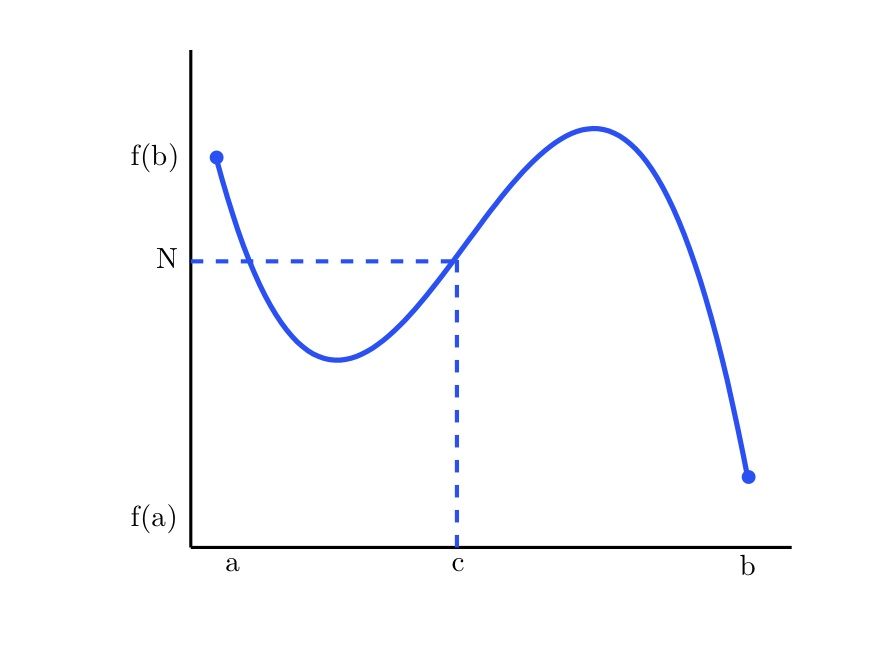
\includegraphics[height=2in]{ivt}
  \caption{figure stolen from Google images} % caption for first subfigure
  \label{fig:IVTgoogleA}  		% label for first subfigure
\end{subfigure}
\begin{subfigure}{.5\textwidth}
  \centering
  \includegraphics[height=2in]{IVT2}
  \caption{figure stolen from Google image} % caption for 2nd subfigure
  \label{fig:IVTgoogleB}  		% label for 2nd subfigure
\end{subfigure}
\begin{subfigure}{.5\textwidth}
  \centering
  \includegraphics[width=2in]{IVT3}
  \caption{figure created in inkscape} % caption for 2nd subfigure
  \label{fig:IVTgoogleC}  		% label for 2nd subfigure
\end{subfigure}
\begin{subfigure}{.5\textwidth}
  \centering
  \includegraphics[height=2in]{IVT4}
  \caption{figure created in inkscape} % caption for 2nd subfigure
  \label{fig:IVTinkscape}  		% label for 2nd subfigure
\end{subfigure}
\caption{Comparison between homemade and stolen images}
\label{fig:IVTsubfigures}
\end{figure}
%
The figure as a whole can be referred to, as well as each subfigure. For example, in figure \ref{fig:IVTsubfigures} I am comparing illustrations which I took form Google images to subfigure \ref{fig:IVTinkscape} which I made myself in inkscape.

\pagebreak

\section{Text wrapping}

Occasionally, it is appropriate to add a small figure in your document and then allow the text to wrap around it. This is useful for popular articles but not recommended for most formal works, or where the figures become too small to read.

\begin{wrapfigure}{r}{0.3\textwidth}
\centering
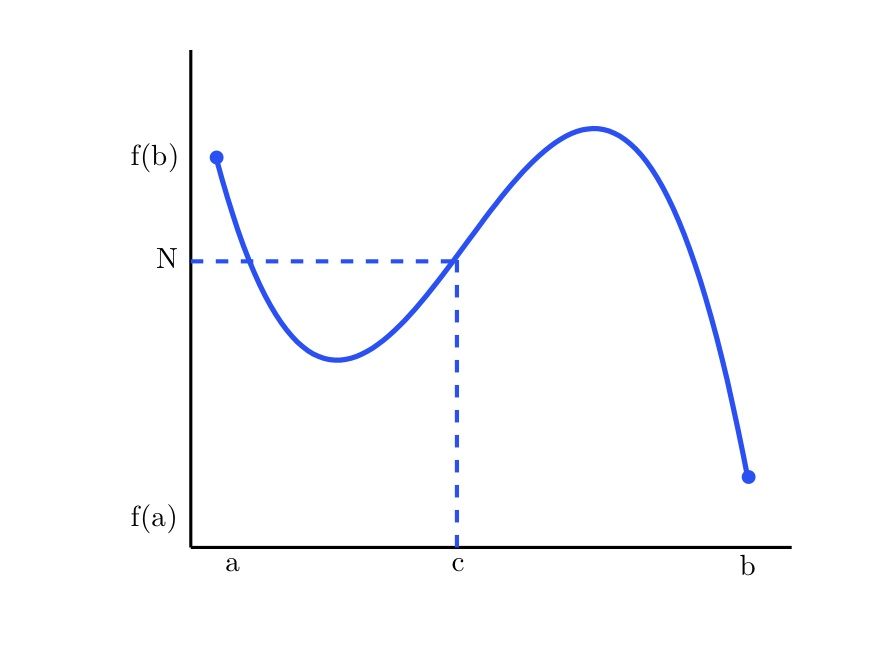
\includegraphics[width=0.28\textwidth]{ivt}
\caption{IVT figure on right of text}
\label{fig:IVTright}
\end{wrapfigure}

To do this we need the wrapfig package  which allows us to change our environment from figure to wrapfigure. this new environment takes in two mandatory arguments, the first argument specifies the position of the figure relative to the surrounding text and thus is usually r or l (to the right/left of the text respectively).
% other options are available, see the wrapfig package documentation https://ctan.org/pkg/wrapfig?lang=en

The second mandatory argument is how much horizontal space should be reserved for the figure. For best results, this should be a little larger than the width of the figure. If this is smaller than the width of the figure, then the figure will overlap the text. If it is too much bigger than the figure, then space is wasted.

blah blah blah blahblah blahblah blahblah blahblah blahblah blahblah blahblah blahblah blahblah blahblah blahblah blahblah blahblah blah
blah blah blah blahblah blahblah blahblah blahblah blahblah blahblah blahblah blahblah blahblah blahblah blahblah blahblah blahblah blah
blah blah blah blahblah blahblah blahblah blahblah blahblah blahblah blahblah blahblah blahblah blahblah blahblah blahblah blahblah blah
%
\begin{wrapfigure}{l}{0.3\textwidth}
\centering
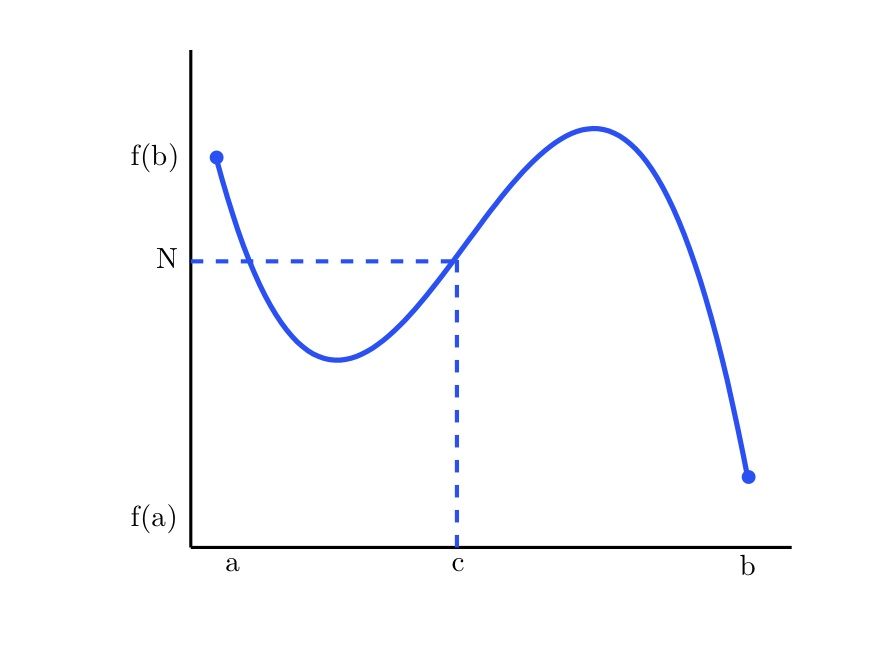
\includegraphics[width=0.28\textwidth]{ivt}
\caption{IVT figure on left of text}
\label{fig:IVTleft}
\end{wrapfigure}
%
yada  yada yadayada yada yadayada yadayadayada yada yadayada yadayada yada yadayada yadayada yada yadayada yadayada yada yadayada yadayada yada  yada  yada yadayada yadayadayada yada yadayada yada yada  yada yadayada yada yadayada yadayadayada yada yadayada yadayada yada yadayada yadayada yada yadayada yadayada yada yadayada yadayada yada  yada  yada yadayada yadayadayada yada yadayada yada yada  yada yadayada yada yadayada yadayadayada yada yadayada yadayada yada yadayada yadayada yada yadayada yadayada yada yadayada yadayada yada  yada  yada yadayada yadayadayada yada yadayada yada yada  yada yadayada yada yadayada yadayadayada yada yadayada yadayada yada yadayada yadayada yada yadayada yadayada yada yadayada yadayada yada  yada  yada yadayada yadayadayada yada yadayada yada yada  yada yadayada yada yadayada yadayadayada yada yadayada yadayada yada yadayada yadayada yada yadayada yadayada yada yadayada yadayada yad

\end{document}
